% vim:encoding=utf8 ft=tex sts=2 sw=2 et:

\documentclass{classrep}
\usepackage[utf8]{inputenc}
\usepackage{color}
\usepackage[sort]{natbib}

\usepackage[pdftex]{graphicx}
\DeclareGraphicsExtensions{.pdf,.png,.jpg,.bmp,.gif}

\usepackage{algorithm}
\usepackage{algorithmic}
\usepackage{mathtools}
\usepackage{indentfirst}
\usepackage[hyphens]{url}
\usepackage[stable]{footmisc}
\usepackage{hyperref}

\usepackage[polish]{babel}
\usepackage[center,small,bf]{caption}
\hypersetup{colorlinks=false,pdfborder={0 0 0}}

\studycycle{Informatyka, studia dzienne, mgr II st.}
\coursesemester{I}

%\coursename{Angelologia teoretyczna i stosowana}
\coursename{Obliczenia inteligentne}
\courseyear{2010/2011}

\courseteacher{dr inż. Arkadiusz Tomczyk}
\coursegroup{środa, 10:15}

\author{
  \studentinfo{Paweł Musiał}{178726} \and
  \studentinfo{Łukasz Michalski}{178724}
}

\title{Zadanie 1: Identyfikacja znaków zakazu na zdjęciach}
\svnurl{http://serce.ics.p.lodz.pl/svn/labs/oi/adres@rewizja}

\begin{document}
\maketitle



\section{Cel}
Zaprojektowanie aplikacji udostępniającej interfejs do identyfikacji obszarów na zdjęciach w których występują znaki zakazu. Na wyjściu interfejs ma za zadanie podać maski wykrytych znaków.

\section{Wprowadzenie}
\textbf{DO POPRAWY!!!!!}
Projekt został podzielony na dwie zasadniczo oddzielne fazy. Pierwszą z nich jest zidentyfikowanie potencjalnych obszarów na których występują poszukiwane znaki. Zadanie to zostało zrealizowane przy pomocy ,,...czegoś takiego co działa...bo Hough Transform nie umiemy używać :]...''. Dzięki której mamy wyznaczone obszary gdzie potencjalnie możemy szukać interesujących nas znaków. Kolejnym etapem jest stwierdzenie czy na znalezionym obszarze znajduje się znak zakazu, etap ten w swojej rdzennej części realizowany jest za pomocą sieci neuronowych, w zadaniu porównano działanie sieci wielowarstwowego perceptronu \footnote{ang. Multilayer Perceptron (MLP)} oraz sieci o radialnej funkcji bazowej \footnote{ang. Radial Basis Function Network (RBF)}.

\subsection{Wyznaczanie obszarów ,,zainteresowania''}

\subsection{Rozstrzyganie czy na obszarze znajduje się znak}




\subsubsection{Ekstrakcja Cech} 
\label{cfseval}
Dane które otrzymujemy z poprzedniego etapu przetwarzania zdjęcia, są zbiorem przeskalowanych do pewnego rozmiaru wycinków zdjęcia. Jednak nawet obraz możliwie mały np 20x20px daje wynikowo wektor 400 danych wejściowych co znacznie spowolniłoby proces nauki jak i również działanie klasyfikatora wynikowego który byłby w dużym stopniu skomplikowany. Aby uzyskać jak najwięcej ważnych informacji z obecnie rozpatrywanego obszaru, jednocześnie  zmniejszając ilość informacji do możliwie najmniejszego podzbioru danych pozwalających na prawidłową ocenę. Użyto algorytmu wybierającego podzbiór cech które w najwyższym stopniu są skorelowane wewnątrz pewnej klasy, jednocześnie pozostając niezależne dla innych klas. Działanie to nie tylko ma na celu zmniejszenie wymiarowości danych, ale jednocześnie - nie jako efekt uboczny, usuniemy cechy które mogłyby pozostawać skorelowane z każdą z klas lub odwrotnie być niezależnymi od każdej klasy,  co w najgorszym przypadku mogłoby prowadzić do pogorszenia wyników klasyfikacji wyuczonym modelem.

Zachłannym podejściem realizującym to zadanie byłoby wybieranie każdego podzbioru cech i określenie jego stopnia przydatności, takie podejście już przy podanym tutaj przykładzie wektora 400 danych, byłoby nie lada wyzwaniem.\\ 
Algorytm użyty w projekcie, a przedstawiony w \cite{Hall1998} oparty jest na wyszukiwaniu heurystycznym najlepszego podzbioru cech - nie przeszukujemy całej przestrzeni możliwych podzbiorów. 
\begin{algorithm}
\caption{wyszukiwanie heurystyczne - BestFirst}
\label{bestfirst}
\begin{algorithmic}[1]
\STATE zbiór Otwarty zawiera stan początkowy, zbiór Zamknięty jest pusty
\STATE \textbf{BEST} $\leftarrow$ początkowy podzbiór
\STATE \textbf{S} $\leftarrow$ argmax(x) (stan ze zbioru Otwartego z najwyższą wagą)
\STATE usuń \textbf{S} ze zbioru Otwarty, dodaj do Zamknięty
\IF{$e(\textbf{S}) \geq e(\textbf{BEST}) $}
\STATE \textbf{BEST} $\leftarrow$ \textbf{S}
\ENDIF
\STATE dla każdego potomka \textbf{t} stanu \textbf{S}, którego nie ma w zbiorach Otwarty i Zamknięty oblicz jego wagę i dodaj do Otwarty
\IF{\textbf{BEST} uległ zmianie idź do kroku 2}
\STATE \textbf{BEST} $\leftarrow$ \textbf{S}
\ELSE
\STATE zwróć \textbf{BEST}
\ENDIF
\end{algorithmic}
\end{algorithm}

W powyższym algorytmie ocena $e(s)$ aktualnego zbioru określona na podstawie korelacji cech względem klas. Zależność tą można przedstawić w następujący sposób:
\begin{equation}
M_{S} = \frac{k r_{ef} }{k + k(k-1)r_{ff} }
\end{equation}
Gdzie :
\begin{itemize}
\item k - liczba cech
\item $r_{ef}$ średnia korelacja między cechami a klasami ($f \in S$)
\item $r_{ff}$ interkorelacja
\end{itemize}
Dokładny opis metody można poznać w \cite{Hall1998}.


\subsubsection{Sieć Wielowarstwowy perceptron\footnote{ang. MLP - Multilayer Perceptron}}
\label{MLP}

Jak nazwa wskazuje jest to sieć wielowarstwowa, czyli składająca się z wielu neuronów połączonych w sieć. Podstawową i najczęściej stosowaną architekturą jest zastosowanie sieci trój warstwowej .

\begin{figure}[H]
\centering
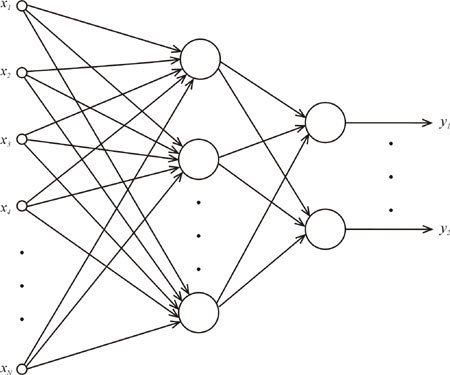
\includegraphics[width=0.4\textwidth]{arch_jw}
  \caption{Schemat trój warstwowej  sieci neuronowej.}
  \label{MLParch}
\end{figure}

Jak na rysunku \ref{MLParch} widać  sieć ta składa się standardowo z warstwy wejściowej propagującej poszczególne składowe na neurony warstwy ukrytej - neurony nieliniowe, w warstwie ukrytej używamy neuronów sigmoidalnych o funkcji przejścia :
\begin{itemize}
\item 
\begin{equation}
f(x) = \frac{1}{1+ e ^{- \beta x }}
\end{equation}
\item 
\begin{equation}
f(x) = \frac{1- e ^{- \beta x }}{1+ e ^{- \beta x }}
\end{equation}
\end{itemize}
Wyjście każdego z tych neuronów obliczamy jako :
\begin{equation}
y(t) = f \left( \sum \limits ^{n} _{i=1} w_{i}(t) x_{i} (t) \right)
\end{equation}
Ostatnią warstwą jest warstwa wyjściowa dająca odpowiedź sieci na wektor wejściowy.\\
Zadanie które ma na celu sieć, jest minimalizacja błędu 
\begin{equation}
Q = \frac{1}{2} \left[ d - f \left( \sum \limits ^{n} _{i=0} w_i x_i \right)  \right] ^{2}
\end{equation}
gdzie $d$ - oczekiwane wyjście sieci.\\

Najpopularniejszym i zarazem najprostszym algorytmem nauki takiej sieci jest algorytm wstecznej propagacji błędu, w najprostszym ujęciu polegający na propagacji błędu na coraz głębsze warstwy sieci względem błędu obliczonego na wyjściu.
Poniżej opis analityczny tego zadania.
\begin{equation}
\label{backprop-error}
Q ^{k} _{i} (t)  = \left\{ 
   \begin{array}{l l}
     d^{L} _{i}(t) - y^{L} _{i}(t) & \quad \text{dla $k=L$}\\
     \sum \limits ^{N_{k+1}} _{m=1} \delta ^{k+1}_{m}(t) w^{k+1} _{mi}(t) & \quad \text{dla $k \in (1,L-1)$}\\
   \end{array} \right.
\end{equation}
\begin{equation}
\delta ^{k+1}_{i}(t) = \varepsilon ^{k} _{i} f' \left( \sum \limits ^{N _{k-1}} _{j=1} w^{k} _{ij}(t) x^{k} _{j} (t) \right) 
\end{equation}
gdzie $\varepsilon ^{k} _{i}$ jest błędem i-tego neuronu w k-tej warstwie
\begin{equation}
\label{backprop-weigh}
w^{k} _{ij} (t+1) = w^{k} _{ij} (t) + 2 \eta \delta ^{k}_{i}(t) x^{k} _{j} (t)
\end{equation}
W powyższym opisie algorytmu nauki sieci wielowarstwowej indeksy (t) oznaczają kolejne iteracje, $N_k$ liczbę neuronów w k-tej warstwie $\eta$ parametr nauki sieci.\\
Sygnał w sieci propagowany jest w warstwy $k$ na $k+1$ gdzie wejściem warstwy $k+1$ jest wyjście z warstwy $k$ $y^{k} _{i}$. Po przejściu sygnału przez siec, to znaczy obliczeniu sygnału wyjściowego obliczanym błąd zgodnie ze wzorem \ref{backprop-error} a następnie propagując go wstecznie na poprzednie warstwy (z warstwy $k$ na warstwę $k-1$). Równocześnie następuje dostosowanie wektorów wag zgodnie z regułą \ref{backprop-weigh}.

Z iteracji na iteracje jeśli sieć będzie miała dobrą architekturę, błąd na wyjściu sieci będzie się minimalizował, w najlepszym przypadku błąd może wynieść 0 czyli bezbłędnie nauczony zbiór uczący, lecz taki wynik tylko powierzchownie może wydać się dobrym. Ponieważ oznaczać to może, że sieć dopasowała się dokładnie do danych uczących i jedynie do danych uczących tym samym nie posiada zdolności generalizacji co w przypadku zadania rozpoznawania wzorców jest efektem niepożądanym gdyż sieć będzie bardzo wrażliwa na zaszumione dane.


\subsubsection{sieć o radialnej funkcji bazowej \footnote{ang. RBF - Radial basis function}}
\label{RBF}

Odmienną koncepcję do uprzednio zaprezentowanej sieci jest zastosowanie nieliniowego przekształcenia przestrzeni danych wejściowych przez wprowadzenie warstwy neuronów ukrytych realizujących funkcję zmieniającą się radialnie wokół wybranego centrum. Neuron radialny jest naturalnym uzupełnieniem neuronu sigmoidalnego, ponieważ umożliwia w przypadku wystąpienia symetrii kołowej danych znaczne uproszczenie sieci, zmniejszenie liczby potrzebnych neuronów w warstwie ukrytej do realizacji zadania klasyfikacji. Neuron sigmoidalny w przestrzeni wielowymiarowej rozdzielał dwie klasy za pomocą hiperpłaszczyzny, w przypadku neuronu radialnego podział dokonywany jest za pomocą podziału kołowego wokół punktu centralnego.
\begin{equation}
\phi (x,c) = \exp \left( \frac{\| x-c \| ^{2}}{2 \sigma ^{2}} \right)
\label{RBFGauss}
\end{equation}
Funkcja radialna - funkcja Gaussa \ref{RBFGauss}.
gdzie :
\begin{itemize}
\item x wektor danych uczących
\item c centrum funkcji radialnej
\end{itemize}

Sieć radialną podobnie jak wielowarstwowy perceptron składa się z trzech warstw wejściowej, ukrytej i wyjściowej. Gdzie w warstwie ukrytej znajdują się neurony o radialnej funkcji bazowej, wejściowe i wyjściowe neurony liniowe. W warstwie ukrytej ilość neuronów powinna zachowana w proporcji $H < N$, gdzie N to liczba neuronów w warstwie wejściowej, ponieważ jeśli nie zachowamy tej zależności sieć będzie dopasowywać do różnego rodzaju szumów i nieregularności występujących w danych - straci zdolność uogólniania. Każdy z nich swoje centrum $c_{h}$, centra te są inicjowane przy tworzeniu struktury sieci, a następnie dopasowywane do danych uczących w trakcie uczenia się sieci.

Problem ten możemy wyrazić jako minimalizacja wyrażenia 
\begin{equation}
E = \sum \limits ^{p} _{i=1} \left[ \sum \limits ^{K} _{j=1} w_j \phi ( x_i c_j) -y_i  \right] ^{2}
\end{equation}

gdzie :
\begin{itemize}
\item x - wektor danych wejściowych
\item w - wektor wag
\item y - oczekiwane wyjście sieci
\item p - liczba wzorców uczących
\item K - liczba neuronów radialnych
\end{itemize}
Algorytm uczenia sieci składa się z dwóch faz. W fazie pierwszej następuje dobór położenia oraz kształt funkcji bazowych za pomocą np : metody k-średnich\footnote{ang. k-means}, metody wstecznej propagacji błędu. Kolejnym krokiem jest dobór macierzy wag która jest wyznaczany za pomogą metody pseudoinwersji macierzy Greena postaci :
\begin{equation*}
G =
\begin{bmatrix}
        \phi (x_1,c_1) & \phi (x_1,c_2) & \cdots  & \phi (x_1,c_H)\\
        \phi (x_1,c_1) & \phi (x_1,c_2) & \cdots  & \phi (x_2,c_H)\\
        \vdots & \vdots & \ddots  & \vdots \\
        \phi (x_N,c_1) & \phi (x_N,c_2) & \cdots  & \phi (x_N,c_H)\\
\end{bmatrix}
\end{equation*}

\begin{equation}
w = G^{+}d(X)
\end{equation}
gdzie : w - wektor wag, d(X) - wektor wartości oczekiwanych dla zbioru X.

Sieci radialne wymagają zazwyczaj użycia większej liczby neuronów niż sieci jednokierunkowe o sigmoidalnej funkcji aktywacji. Pomimo to, uczenie ich trwa o wiele której niż w przypadku sieci perceptronowych. Na ogół uważa się, że sieci o radialnych funkcjach bazowych nadają się lepiej do zadań klasyfikacji takich jak rozpoznawanie wzorców. 


\subsubsection{Algorytm AdaBoost \footnote{ ang Adaptive Boosting - wzmacnianie adaptacyjne} }
\label{AdaBoostSec}
Jest to algorytm wzmacniania klasyfikatorów. Metoda ta buduje rodzinę słabych klasyfikatorów których ważona decyzją daje werdykt o ostatecznej przynależności do klasy. 

\begin{algorithm}[h]
\caption{AdaBoost}
\label{adaboost}
\begin{algorithmic}[1]
\STATE Ustalenie wektora wag w, następujący sposób $w^{1} _{j} \in [0,1] \implies \sum \limits ^{n} _{j=1} w^{1} _{j} = 1$
\FOR{$i = 1 \to B$} 
\STATE pobierz próbę bootstrapową $\zeta ^{*b} _{n}$ z próby $\zeta _{n}$ według rozkładu 
\[ P(z_{j} \in \zeta ^{*b} _{n} ) = w ^{b} _j \]
\STATE konstruuj klasyfikator $\hat{d}_b$ dla próby  $\zeta ^{*b} _{n}$
\STATE oblicz $\hat{e} _{b} = \sum \limits ^{n} _{j=1} w^{b} _{j} l ^{b} _{j}$, gdzie
\[
l ^{b} _{j}  = \left\{ 
   \begin{array}{l l}
     1 & \quad \text{jesli $\hat{d}_b(x_j) \neq y_j$}\\
     0 & \quad \text{jesli $\hat{d}_b(x_j) = y_j$}\\
   \end{array} \right.
   \]
\IF{$\hat{e}_{b} \in (0; 0.5)$}
\STATE
\[
\beta _{b} = \frac{\hat{e} _{b}}{1 - \hat{e} _{b}}
\]
\ELSE
\STATE $w^{b} _{j} = \frac{1}{n}$ a następnie wróć do 3.
\ENDIF
\STATE aktualizuj wagi
\[
w^{b+1} _{j} = \frac{w^{b} \beta ^{1-l^{b} _{j}} _{b}}{\sum \limits ^{n} _{i=1} w ^{b} _{i} \beta ^{1-l ^{b} _{i}} _{b}}
\]
\ENDFOR
\STATE Klasyfikuj obserwacje x wg reguły
\[
\hat{d} _{AdaBoost} (x)= arg max \sum \limits ^{B} _{b=1} \left[ ln \left( \frac{1} {\beta _{b}}  \right) I \left( \hat{d}_b (x) = k \right) \right]
\]
\end{algorithmic}
\end{algorithm}


W algorytmie tym, każdy kolejny klasyfikator zależy od uprzednio skonstruowanego. W b-tej iteracji w kroku 5 obliczany jest poziom błędu klasyfikatora $\hat{d}_{b}$ , a następnie wyznaczane wielkości $\beta _b $ wykorzystywane w aktualizacji wag. Poziom błędu jest jest zależny od wag, ponieważ jest ważoną sumą, a nie frakcją obserwacji błędnie zaklasyfikowanych.  Wagi obserwacji błędnie zaklasyfikowanej przez $\hat{d}_{b}$ są zwiększane, a poprawnie zaklasyfikowanych zmniejszane, w ten sposób wzrasta prawdopodobieństwo, z jakim obserwacja klasyfikowana błędnie przez klasyfikator $\hat{d}_{b}$ zostanie wylosowana jako element próby uczącej klasyfikatora $\hat{d}_{b+1}$. Również klasyfikatory składowe o większej poprawności predykcji mają większy udział w ostatecznej decyzji klasyfikatora łączonego. Nowo zaobserwowany obiekt zostaje przydzielony do grupy $k$, jeżeli suma wag klasyfikatorów składowych identyfikujących go jako obiekt grupy $k$ jest największa.  


\section{Opis implementacji}


\subsection{Rozstrzyganie czy na obszarze znajduje się znak}
W implementacji tej części głównie posiłkowano się biblioteką przeznaczoną do zadań związanych z analizą danych \cite{weka}. W bibliotece tej zawarte są klasy implementujące wszystkie opisane metody użyte w tej części programu. 

\begin{itemize}
\item \textit{\color{blue}weka.attributeSelection.CfsSubsetEval}  - implementacja opisanej w sekcji \ref{cfseval} metody wyznaczania podzbioru cech najbardziej znaczących
\item \textit{\color{blue}weka.attributeSelection.BestFirst} - algorytm wyszukujący używany przez metodę ewaluacji optymalnego podzbioru, opisanego w pseudokodzie \ref{bestfirst}
\item \textit{\color{blue}weka.classifiers.functions.MultilayerPerceptron} - implementacja sieci wielowarstwowego perceptronu opisanej w \ref{MLP}
\item
\textit{\color{blue}weka.classifiers.functions.RBFNetwork} - implementacja sieci o radialnej funkcji bazowej opisanej w \ref{RBF} 
\item \textit{\color{blue}weka.classifiers.meta.AdaBoostM1} - implementacja metody wzmacniania klasyfikatorów opisanej w \ref{AdaBoostSec}

\end{itemize}


\section{Materiały i metody}


\subsection{Rozstrzyganie czy na obszarze znajduje się znak}
Do nauki klasyfikatorów należało zebrać odpowiedni zbiór uczący zawierający dane będące wzorcami umożliwiającymi poprawną klasyfikacje obszarów zawierających znaki zakazu. Zbiór ten powstał na podstawie posiadanych naturalnych zdjęć robionych z drogi, następnie wycinano obszary zdjęć gdzie znajdowały się znaki zakazu, ostrzegawcze, informacyjne, nakazu, aby zebrać odpowiednio duże zbiory przykładów pozytywnych i negatywnych do nauki. Z powodu małej ilości zarejestrowanych znaków odwołania ograniczeń - przypadek znaków zakazu, stworzono zbiór sztuczny na podstawie szkiców tych znaków, które następnie zostały zaszumione różnymi rodzajami szumów oraz rozmyte przy pomocy rozmycia gaussa lub rozmycia ,,w ruchu''. Przekształcenia danych zostały wykonane przy pomocy biblioteki graficznej ImageMagick++ \footnote{\url{www.imagemagick.org}}.

\section{Wyniki}

\subsection{Rozstrzyganie czy na obszarze znajduje się znak}

W sekcji ten zostaną przedstawione wyniki klasyfikacji zbioru 86 obrazów składającego się z : 6 obrazów sztucznych reprezentujących znaki odwołania ograniczeń, oraz 80 obrazów znaków naturalnych z czego 20 zawierają znaki zakazu inne od znaków odwołania.
Stosowane oznaczenia :\\
Klasy :
\begin{itemize}
\item positive0 - znak zakazu (bez odwołań)
\item positive1 - znak zakazu (tylko odwołania)
\item negative - znaki ostrzegawcze, nakazu, informacyjne
\end{itemize} 
TP - ang. True Positive, prawidłowe rozpoznanie klasy.\\
FP - ang. False Positive, nietrafne rozpoznanie klasy.\\
Precision - stosunek prawidłowo rozpoznanych obiektów klasy do wszystkich obiektów przydzielonych do tej klasy(TP+FP).\\
Recall - stosunek prawidłowo rozpoznanych obiektów klasy do obiektów należących do klasy.


\subsubsection{sieć Wielowarstwowy perceptron}

\begin{table}[H]
\centering
\begin{tabular}{|c|c|c|}
\hline 
Poprawnie zaklasyfikowanych & 73 & 84.88\% \\ 
\hline 
Niepoprawnie zaklasyfikowanych & 13 & 15.11\% \\ 
\hline 
\end{tabular} 
\caption{Dokładność metody MLP.}
\label{wyniki:mlpproc}
\end{table}



\begin{table}[H]
\centering
\begin{tabular}{|c|c|c|c|c|}
\hline 
TP Rate &  FP Rate & Precision &  Recall &  Klasa \\
\hline
0.8    &   0.136   &   0.64  &    0.8  &  positive0 \\
\hline
1      &   0     &     1    &     1   &   positive1 \\
\hline
0.85    &  0.154  &    0.927  &   0.85  & negative \\
\hline 
\end{tabular} 
\caption{Wyniki klasyfikacja dla poszczególnych klas, metodą MLP.}
\label{wyniki:mlpclass}
\end{table}


\subsubsection{sieć o radialnej funkcji bazowej}


\begin{table}[H]
\centering
\begin{tabular}{|c|c|c|}
\hline 
Poprawnie zaklasyfikowanych & 79 & 91.86\% \\ 
\hline 
Niepoprawnie zaklasyfikowanych & 7 & 8.13\% \\
\hline 
\end{tabular} 
\caption{Dokładność metody RBFN.}
\label{wyniki:rbfproc}
\end{table}



\begin{table}[H]
\centering
\begin{tabular}{|c|c|c|c|c|}
\hline 
TP Rate &  FP Rate &  Precision &  Recall &  Klasa\\
\hline
0.7    &   0.015  &    0.933  &   0.7 &    positive0\\
\hline
1      &   0     &     1   &      1   &    positive1\\
\hline
0.983  &   0.231   &   0.908  &   0.983  & negative\\
\hline 
\end{tabular} 

\caption{Wyniki klasyfikacja dla poszczególnych klas, metodą RBFN.}
\label{wyniki:rbfclass}
\end{table}


\section{Dyskusja}


\subsection{Rozstrzyganie czy na obszarze znajduje się znak}
Jak widać już na ogólnym zestawieniu procentowym udanych klasyfikacji \ref{wyniki:mlpproc} \ref{wyniki:rbfproc}, zgodnie z oczekiwaniami sieć o radialnej funkcji bazowej poradziła sobie znacznie lepiej od sieci wielowarstwowego perceptronu. Oraz, czego tutaj nie zestawiono, klasyfikator o radialnej funkcji bazowej był znacznie bardziej złożony od odpowiednika perceptronu. Jednak jak widać w zestawieniach trafności poszczególnych klas \ref{wyniki:mlpclass}, \ref{wyniki:rbfclass} klasyfikator zbudowany na neuronach o radialnej funkcji bazowej znacznie lepiej potrafi klasyfikować znaki zakazu mówią nam o tym dokładnie zestawione wskaźniki. Chociażby bardzo ważny \emph{FP} który w przypadku MLP miał wartość 0.136 a dla RBF zaledwie 0.015.


\section{Wnioski}

\subsection{Rozstrzyganie czy na obszarze znajduje się znak}
W części tej udało się stworzyć klasyfikator którego zdolności klasyfikacji są zadowalające, wynik powyżej 90\% wydaje się być akceptowalnym, z tym rodzaju zadania przy tak małym przetworzeniu danych - działamy praktycznie na danych naturalnych. Jednak z drugiej strony zbiór testowy był bardzo mały aby stwierdzić, czy sprawność zbudowanego modelu utrzymała by się na zaobserwowanym przez nas poziomie należałoby by zebrać wystarczająco zróżnicowany zbiór modelujący nam w pewnym stopniu prawdopodobne różnicowanie obrazów wejściowych na których mielibyśmy za zadanie zidentyfikowanie znaków. 


\bibliographystyle{plainnat}
\bibliography{bibliografia}


\end{document}
